\section {Η Περιπέτεια (The Adventure)}
%
Ότι έχουμε δει ως εδώ είναι μια μικρή εισαγωγή στον προγραμματισμό και την
python. Πιο πολύ βέβαια είναι μια συνειδητή προσπάθεια από μέρους
μας να σας ωθήσουμε υποσυνείδητα στον προγραμματισμό. Θυμηθείτε: κάθε φορά
που τρέχετε ένα πρόγραμμα στον υπολογιστή, εκτελείτε κάτι που δημιουργήθηκε
από κάποιον άλλο. Γιατί όχι από εσάς; Αν ο υπολογιστής είναι μια
προγραμματιζόμενη μηχανή γενικής χρήσης, γιατί πρέπει εμείς να αφήσουμε το
``προγραμματιζόμενη'' στους άλλους; Μήπως είναι καλύτεροι από εμάς;
Δεν σας κρύβω ότι όλοι εμείς που ξεκινήσαμε πολύ παλιά τον
προγραμματισμό, είχαμε τα πλεονεκτήματα της αμεσότητας και απλότητας των
μηχανημάτων. Επίσης δεν είχαμε και τίποτα άλλο να κάνουμε με αυτά! Εξ'
αρχής, τα είχαμε αγοράσει για να μάθουμε προγραμματισμό. Τώρα όμως, μέσα στο
πλήθος των πληροφοριών, οι υπολογιστές έχουν υποβιβαστεί σε συσκευές. Έχουμε
όλοι γυρίσει στα έτοιμα πράγματα ενώ έχουμε σημαντικά νέα πλεονεκτήματα:
Γρήγορα μηχανήματα, τεράστιες μνήμες, αφθονία ελεύθερων γλωσσών
προγραμματισμού και φυσικά το Internet για να ψάχνουμε! Φαίνεται όμως ότι η
πολύ αφθονία βλάπτει.

Ευτυχώς, υπάρχει η python και φυσικά το βιβλίο που κρατάτε στα χέρια σας!
Γιατί θα φέρουμε κάτι από αυτή τη χαμένη αμεσότητα πίσω, γράφοντας τα παλιά
καλά (θεός να τα κάνει) παιχνίδια στη σύγχρονη εκδοχή τους. Τα πλεονεκτήματα
θα είναι πολλά:
%
\begin{itemize}
\item Θα μάθετε να σκέφτεστε σαν προγραμματιστής (βασικά, θα μάθετε να σκέφτεστε.  Τελεία.)
\item Θα μάθετε λίγη python και pygame για να συνεχίσετε να γράφετε δικά σας παιχνίδια και παραλλαγές αυτών που θα σας δείξουμε.
\item Θα κολλήσετε τόσο άσχημα με τον προγραμματισμό, που θα μένετε όλη μέρα σπίτι σας, δεν θα απαντάτε στο τηλέφωνο και θα τρέφεστε αποκλειστικά με πίτσες,
καφέδες και αναψυκτικά τύπου κόλα.
\end{itemize}
%
ΟΚ, το τελευταίο ίσως δεν είναι ιδιαίτερα καλό αλλά είμαστε σίγουροι ότι
μπορείτε να το ελέγξετε.  Πριν συνεχίσετε να διαβάζετε το κεφάλαιο,
βεβαιωθείτε ότι έχετε κάνει και κατανοήσει τις ασκήσεις του πρώτου
κεφαλαίου και φυσικά τα παραδείγματα με τις λίστες που παρουσιάσαμε
προηγουμένως. Θα τα χρειαστούμε άμεσα.
%
\subsection{Εισαγωγή στις Περιπέτειες Κειμένου (Text Adventures)}
%
Μη σας φαίνεται απίστευτο, το δεύτερο μας παιχνίδι --- αισθητά μεγαλύτερο από
το number guess --- είναι ένα παιχνίδι περιπέτειας. Όχι μη πάει ο νου σας σε
κάτι με τρισδιάστατα γραφικά τύπου Final Fantasy! (αυτό θα το γράψετε εσείς,
μετά που θα διαβάσετε αυτό και πολλά(!) ακόμα βιβλία). Ένα adventure στην απλούστερη του μορφή περιέχει μόνο κείμενο. Τα λεγόμενα {\em text adventures} ήταν πολύ της μόδας πριν μερικές δεκαετίες. Βλέπετε, υπήρχαν τότε υπολογιστές που δεν μπορούσαν να δείξουν παρά μόνο κείμενο στις οθόνες τους (όσο σοκαριστικό και αν ακούγεται αυτό!) Αλλά και εκείνοι που μπορούσαν να δείξουν γραφικά, ε δεν ήταν ακριβώς και\ldots{} φωτογραφικής ποιότητας. Σε κάθε περίπτωση επειδή ο προγραμματιστής δεν ήταν απαραίτητα και γραφίστας, τα text adventures κυριαρχούσαν.

Η ιδέα πίσω από ένα adventure κειμένου είναι ότι ο παίκτης ξεκινάει σε ένα
δωμάτιο. Ο υπολογιστής τυπώνει μια περιγραφή του χώρου με τις πιθανές
εξόδους (πόρτες, σκάλες κλπ) και ο παίκτης αποφασίζει την επόμενη του
κίνηση. Όταν εισέρχεται σε ένα νέο δωμάτιο, η διαδικασία επαναλαμβάνεται,
μέχρι είτε ο παίκτης να κερδίσει (π.χ. να βρει το αντικείμενο που είναι ο
στόχος του παιχνιδιού ή να φτάσει στο κατάλληλο δωμάτιο) είτε να χάσει (να
τον πιάσει το τέρας, το alien ή η μαμά του -- που ορισμένοι θεωρούν χειρότερο
τέλος και από το alien). Σε μερικά adventures υπάρχουν περισσότεροι από ένας
τρόποι για να κερδίσει κανείς και σίγουρα υπάρχουν πολλοί τρόποι να χάσει!
Σε πιο εξελιγμένες μορφές, ένα text adventure απαιτεί από το χρήστη να
συλλέγει αντικείμενα τα οποία θα χρειαστεί σε άλλα δωμάτια. Και φυσικά
χρησιμοποιούνται περισσότερες εντολές για να εκπληρώσουν αυτό το σκοπό.

Το adventure που θα γράψουμε εμείς βασίζεται στο πρωτότυπο που είχε
δημοσιευθεί στο άρθρο ``Παιχνίδια Περιπέτειας'' του Στάθη Ευθυμίου στο
περιοδικό Pixel τον Ιανουάριο του 1986! Χρησιμοποιούμε τον ίδιο χάρτη και
τις πρωτότυπες περιγραφές των δωματίων, αλλά φυσικά το γράφουμε σε python
και όχι σε BASIC.

\begin{SCfigure}
  \centering
  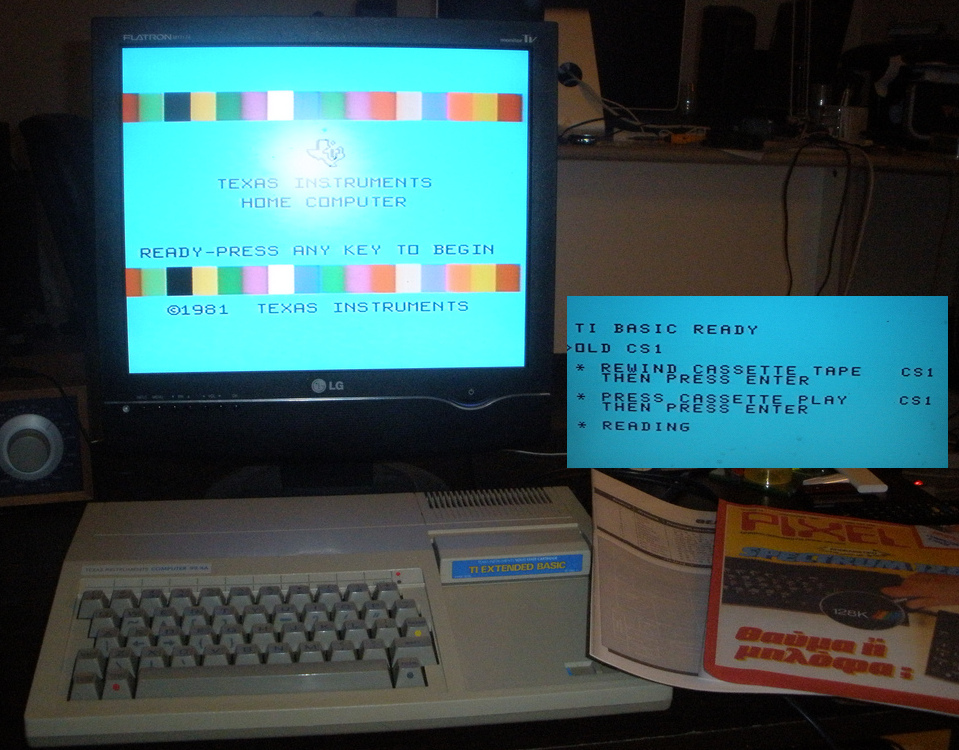
\includegraphics[width=0.4\textwidth]{images/chapter2/ti99-2}
  \caption[TI-99/4A: Από το Χρονοντούλαπο]{Το μηχάνημα στο οποία έγραψα --- το 1986 --- την πρώτη έκδοση του προγράμματος που φαίνεται εδώ. Ναι, το ξέθαψα από την ντουλάπα και το φόρτωσα (από την κασέτα όπως φαίνεται δεξιά, μετά από 26 χρόνια!) για χάρη σας! Και ναι, δουλεύει ακόμα. Βλέπετε και τις σελίδες του Pixel με το αντίστοιχο θέμα.}
  \label{2-1}
\end{SCfigure}

\begin{SCfigure}
  \centering
  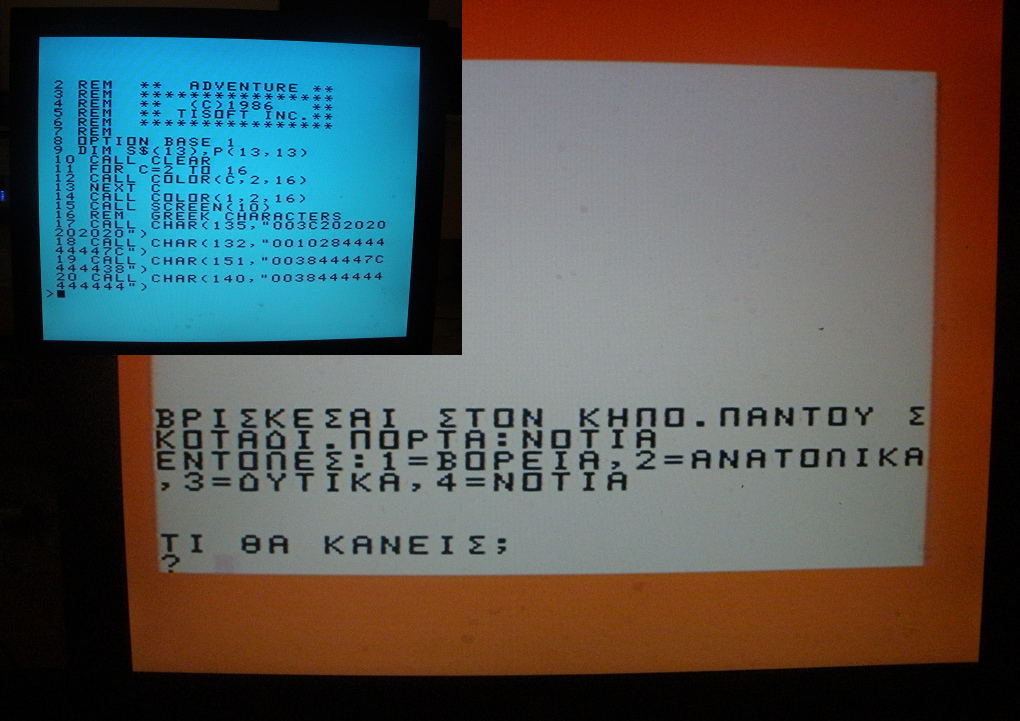
\includegraphics[width=0.4\textwidth]{images/chapter2/adventure-run2}
  \caption[Η Περιπέτεια, το αρχικό listing]{'Ένα μικρό κομμάτι από το listing του αρχικού προγράμματος Adventure, © 1986! Φαίνεται επίσης και η εκτέλεση του προγράμματος όπου βλέπετε ότι δέχεται κατευθύνσεις του τύπου 1,2,3,4.}
 \label{2-2}
\end{SCfigure}

Δεν σας κρύβω ότι διαβάζοντας τότε το άρθρο, άρχισα να σκέφτομαι πως θα
μπορούσα να το υλοποιήσω στον τότε υπολογιστή μου. Υπήρχε βέβαια ένα listing
σε BASIC στο περιοδικό, αλλά εκτός ότι δεν ήταν συμβατό με το δικό μου
μηχάνημα (που βλέπετε στην εικόνα \ref{2-1}), χρησιμοποιούσε και μια λογική που δεν μου άρεσε ιδιαίτερα. Ήμουν σίγουρος ότι μπορούσα να βρω μια πιο ωραία
προγραμματιστικά λύση και πράγματι πέρασα μερικές μέρες σκεπτόμενος το
πρόβλημα σαν ένα background task στο μυαλό μου (κατανάλωνε αρκετούς πόρους
πάντως!) Ένα βράδυ πετάχτηκα από το κρεβάτι έχοντας την απάντηση που
χρειαζόμουν! Η πρώτη έκδοση είχε γραφτεί μέχρι το πρωί\ldots

Ο ίδιος αυτός τρόπος --- αλλά προσαρμοσμένος στα δεδομένα της python ---
παρουσιάζεται εδώ. Όπως θα διαπιστώσετε κατανοώντας το πρόγραμμα, πρόκειται
ουσιαστικά για μια μίνι μηχανή περιπέτειας καθώς μπορείτε να αλλάξετε τα
δεδομένα μέσα στο πρόγραμμα και να δημιουργήσετε μια διαφορετική περιπέτεια.
%
\subsection{Ο Χάρτης}
%
Βασικό σημείο στα text adventures είναι ο χάρτης που δείχνει όλα τα δωμάτια
και τους τρόπους σύνδεσης / επικοινωνίας μεταξύ τους. Το χάρτη αυτό θα
πρέπει να τον φτιάξετε πριν αρχίσετε να γράφετε την περιπέτεια σας. Φυσικά
θα έχετε σκεφτεί και κάποιο συναρπαστικό σενάριο για την περιπέτεια σας ώστε
να έχετε περιγραφές για το κάθε δωμάτιο. Γεγονός είναι ότι επειδή θα έχετε
γράψει εσείς την περιπέτεια μάλλον θα σας είναι εύκολο και να την κερδίσετε.
Αλλά δεν πειράζει, θα παίξουν και οι φίλοι σας.

Ο δικός μας χάρτης παραμένει πιστός στο αρχικό άρθρο και φαίνεται στη εικόνα
\ref{2-3}.

\begin{figure}[H]
  \centering
  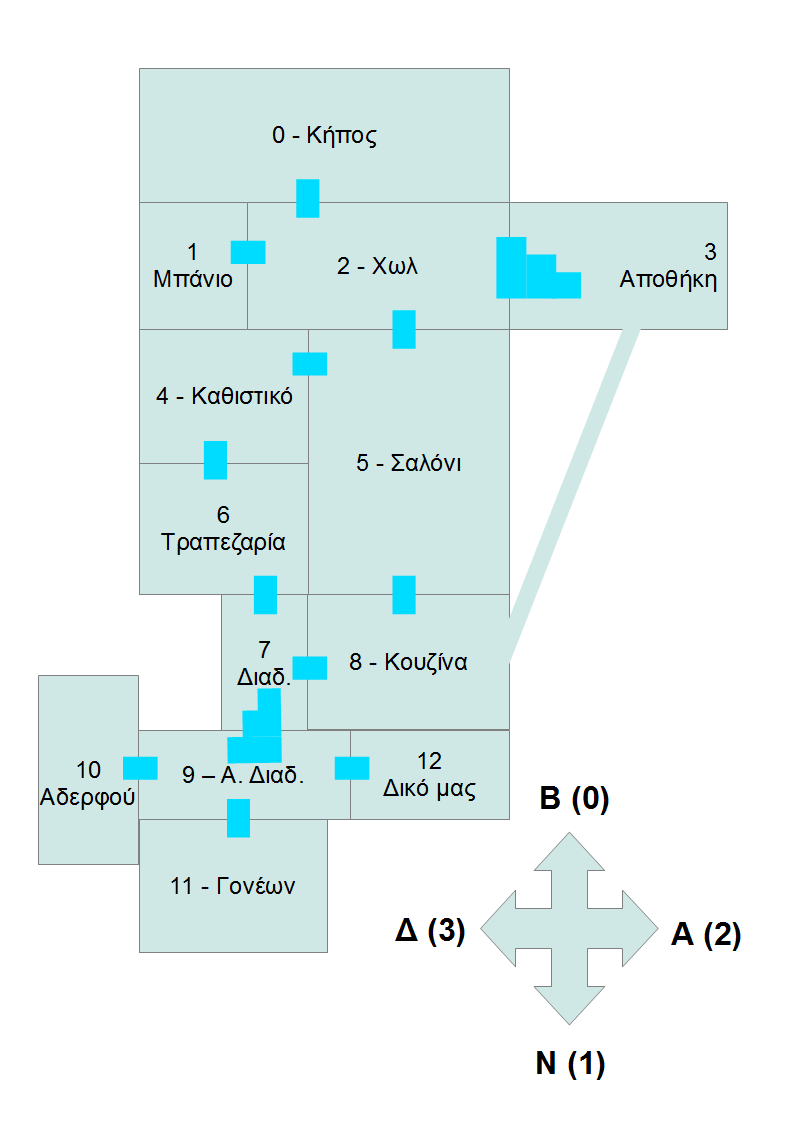
\includegraphics[width=0.4\textwidth]{images/chapter2/adventure-map}
  \caption{Ο Χάρτης της Νυχτερινής Περιπέτειας}
  \label{2-3}
\end{figure}

Πρόκειται προφανώς για ένα μικρού μεγέθους adventure (αλλά μπορείτε με την
ίδια μηχανή να φτιάξετε ένα  όσο μεγάλο θέλετε) και διαδραματίζεται σε ένα
σπίτι με τα παρακάτω δωμάτια/χώρους:

\begin{table}[H]
\begin{center}
\begin{tabular}{|c|l|}
\hline
  \textbf{Αριθμός Δωματίου} & \textbf{Περιγραφή} \\
\hline
0 & Κήπος \\
\hline
1 & Μπάνιο \\
\hline
2 & Χωλ \\
\hline
3 & Αποθήκη \\
\hline
4 & Καθιστικό \\
\hline
5 & Σαλόνι \\
\hline
6 & Τραπεζαρία \\
\hline
7 & Διάδρομος \\
\hline
8 & Κουζίνα \\
\hline
9 & Επάνω διάδρομος \\
\hline
10 & Δωμάτιο Αδερφού \\
\hline
11 & Δωμάτιο Γονέων \\
\hline
12 & Δικό μας Δωμάτιο \\
\hline
\end{tabular}
\end{center}
\caption{Τα δωμάτια της περιπέτειας}
\label{t2-1}
\end{table}

Δώστε έμφαση στο γεγονός ότι έχουμε κωδικοποιήσει τα δωμάτια με αριθμούς από
το 0 ως το 12. Αυτό θα το χρησιμοποιήσουμε φυσικά στο πρόγραμμα και θα μας
διευκολύνει πάρα πολύ.
%
\begin{figure}
  \centering
  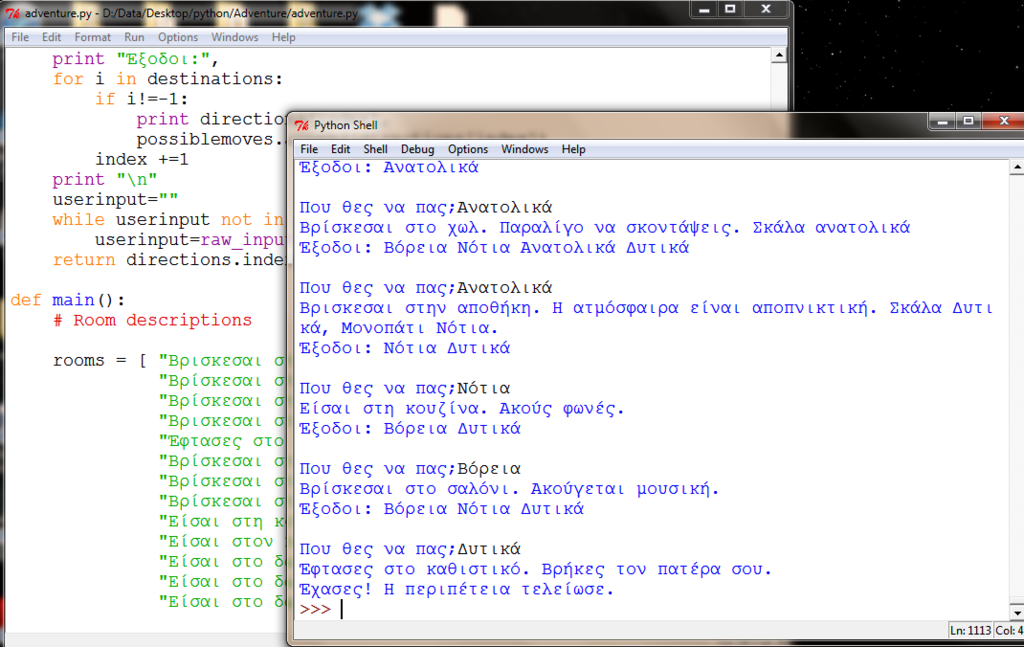
\includegraphics[width=0.8\textwidth]{images/chapter2/py-adventure-run}
  \caption[Εκτέλεση του Adventure]{Η εκτέλεση του προγράμματος στο περιβάλλον της python.}
  \label{2-4}
\end{figure}
%
\subsection{Το Σενάριο}
%
Ο αρχικός συγγραφέας ονόμασε αυτό το παιχνίδι ``Νυχτερινή Περιπέτεια''. Με
απλά λόγια το σενάριο είναι το παρακάτω: Είστε ένας μαθητής, μέλος μιας
οικογένειας με αυστηρές ηθικές αρχές (ξέρετε, από αυτές που τα παιδιά
γυρίζουν πριν τους γονείς στο σπίτι. Πριν νυχτώσει δηλαδή, όχι πριν
ξημερώσει).  Έχετε βγει κρυφά τη νύχτα (!) και τώρα πρέπει να επιστρέψετε
στο σπίτι, στο δωμάτιο σας χωρίς να σας αντιληφθεί κανείς. Θα πρέπει να
αποφύγετε τον πατέρα σας, τη μητέρα σας και τον\ldots{} αδερφό σας που είναι
μαρτυριάρης και θα τα πει όλα! Η μητέρα σας είναι στο δωμάτιο των γονέων, ο
πατέρας σας στο καθιστικό και ο αδερφός σας στο δωμάτιο του. Θα πρέπει να
βρείτε τη διαδρομή για το δωμάτιο σας χωρίς να πέσετε πάνω σε κάποιον από
αυτούς. Φυσικά, υποτίθεται ότι δεν ξέρετε από πριν που είναι ο καθένας! (Μια
ενδιαφέρουσα παραλλαγή θα ήταν να κάνετε το παιχνίδι να τοποθετεί αυτούς
τους χαρακτήρες σε κάποια τυχαία δωμάτια ώστε κάθε φορά που θα το τρέχετε να
είναι διαφορετικό. Βέβαια σε πολλές περιπτώσεις δεν θα υπάρχει  λύση).

Σαν λογική είναι ιδιαίτερα απλό:
%
\begin{enumerate}
\item Ο παίκτης ξεκινάει από το δωμάτιο με αριθμό 0 (κήπος) και του εμφανίζεται η περιγραφή του χώρου και οι πιθανές έξοδοι σε μορφή κατευθύνσεων (π.χ. Νότια).
\item Ο παίκτης δίνει την κατεύθυνση, και εφόσον είναι έγκυρη, το πρόγραμμα τον πηγαίνει στο αντίστοιχο δωμάτιο.
\item Αν ο παίκτης βρεθεί σε δωμάτιο που κερδίζει ή χάνει, τυπώνεται το
αντίστοιχο μήνυμα και η περιπέτεια τελειώνει, διαφορετικά\ldots
\item \ldots{}τυπώνεται η νέα περιγραφή και έξοδοι και επανερχόμαστε στο βήμα 2.
\end{enumerate}
%
Καθώς καταλαβαίνετε το κύριο μέρος του προγράμματος είναι ένας βρόχος του
τύπου:
%
\begin{verbatim}
“Όσο ο παίκτης δεν (έχασε ή κέρδισε)”
\end{verbatim}
%
\subsection{Προγραμματιστική Λογική}
%
\subsubsection{Τα Δωμάτια}
%
Το εύκολο κομμάτι, είναι να κωδικοποιήσουμε τα δωμάτια. Θα χρησιμοποιήσουμε
εδώ μια λίστα της python, την οποία, ευφάνταστα, ονομάσαμε {\tt rooms}:

\begin{minted}[bgcolor=bg, frame=lines, framesep=10pt]{python}
rooms = [  "Βρίσκεσαι στον κήπο. Παντού σκοτάδι.",
           "Βρίσκεσαι στο μπάνιο. Ακούς θόρυβο.",
           "Βρίσκεσαι στο χωλ. Παραλίγο να σκοντάψεις. Σκάλα ανατολικά",
           "Βρίσκεσαι στην αποθήκη. Η ατμόσφαιρα είναι αποπνικτική.\
            Σκάλα Δυτικά, Μονοπάτι Νότια.",
           "Έφτασες στο καθιστικό. Βρήκες τον πατέρα σου.",
           "Βρίσκεσαι στο σαλόνι. Ακούγεται μουσική.",
           "Βρίσκεσαι στην τραπεζαρία. Τα πάντα είναι ανάστατα.",
           "Βρίσκεσαι στο διάδρομο. Είναι σκοτεινά. Σκάλα Νότια",
           "Είσαι στη κουζίνα. Ακούς φωνές.",
           "Είσαι στον πάνω διάδρομο. Παντού ησυχία. Σκάλα Βόρεια.",
           "Είσαι στο δωμάτιο του αδερφού σου. Ο αδερφός σου σε μαρτυρά!",
           "Είσαι στο δωμάτιο των γονέων σου. Η μητέρα σου σε έπιασε.",
           "Είσαι στο δωμάτιο σου. Είσαι ασφαλής." ]
\end{minted}

\begin{SCfigure}
  \centering
  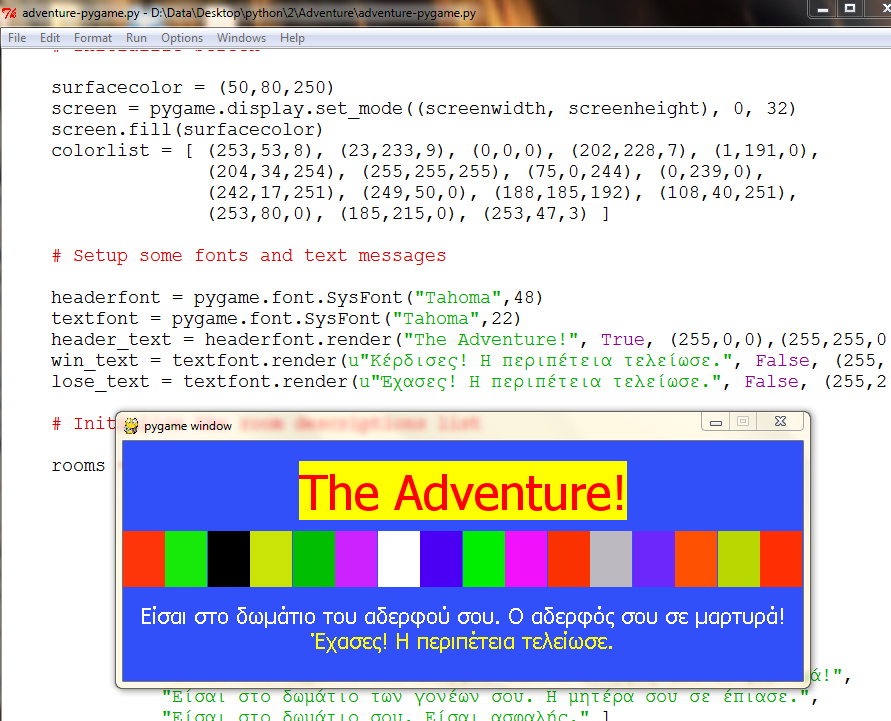
\includegraphics[width=0.7\textwidth]{images/chapter2/py-adventure-pygame-run}
  \caption[Εκτέλεση του Adventure σε pygame]{Επειδή ξέρω ότι θέλετε (εντάξει, πεθαίνετε) να δείτε πως θα ήταν
το παιχνίδι σε ``γραφική'' μορφή, δείτε το μέσω pygame. Η βασική μηχανή είναι
φυσικά ίδια, αλλά ίσως δεν μπορέσετε να κατανοήσετε --- για την ώρα --- το
υπόλοιπο.  Εγκαταστήστε όμως το pygame για να το τρέξετε (για windows δείτε
\url{http://www.pygame.org/download.shtml}, για Linux φυσικά στο repository
της διανομής σας). Κατεβάστε το παιχνίδι από εδώ: \url{http://www.freebsdworld.gr/files/adventure-pygame.zip}}
  \label{2-5}
\end{SCfigure}

Παρατηρήστε ότι έχουμε περάσει τις περιγραφές με την ίδια σειρά (0-12) που
είδαμε πριν. Αυτό μας επιτρέπει να αποθηκεύσουμε το τρέχον δωμάτιο (αυτό στο
οποίο βρίσκεται ο παίκτης την δεδομένη στιγμή) σε μια μεταβλητή που θα
ονομάσουμε {\tt room}. Έτσι, αν ο χρήστης βρίσκεται στο δωμάτιο 2 (το χωλ), οι
παρακάτω εντολές δίνουν την περιγραφή:
%
\begin{verbatim}
room = 2
print rooms[room]

“Βρίσκεσαι στο χωλ. Παραλίγο να σκοντάψεις. Σκάλα ανατολικά”
\end{verbatim}
%
Πιστεύουμε ότι είναι αρκετά απλό να καταλάβετε ότι κάθε φορά το πρόγραμμα θα
δίνει τη σωστή τιμή --- με κάποιο τρόπο που θα δούμε --- στη μεταβλητή {\tt
room} και
θα χρησιμοποιεί την παραπάνω {\tt print} για να τυπώνει το μήνυμα. Αλλά πως θα
κωδικοποιήσουμε την κίνηση από το ένα δωμάτιο στο άλλο;
%
\subsubsection{Οι Κατευθύνσεις και οι Προορισμοί}
%
Δείτε ξανά το σχήμα του χάρτη. Παρατηρήστε στο κάτω μέρος τα βελάκια των
κατευθύνσεων: Έχουμε κωδικοποιήσει κάθε κατεύθυνση με ένα αριθμό: Βόρεια =
0, Νότια = 1, Ανατολικά = 2, Δυτικά = 3. Φανταστείτε τώρα ότι βρίσκεστε στο
δωμάτιο 9 που έχει τέσσερις πιθανές εξόδους:

\begin{table}[H]
\begin{center}
\begin{tabular}{|l|l|}
\hline
  \textbf{Κατεύθυνση} & \textbf{Δωμάτιο Προορισμού} \\
\hline
0 (Βόρεια) & 7 (Διάδρομος \\
\hline
1 (Νότια) & 11 (Δωμάτιο γονέων) \\
\hline
2 (Ανατολικά) & 12 (Δικό μας δωμάτιο) \\
\hline
3 (Δυτικά) & 10 (Δωμάτιο αδερφού) \\
\hline
\end{tabular}
\end{center}
\caption{Κατευθύνσεις και προορισμοί από το δωμάτιο 9}
\label{t2-2}
\end{table}

Αν δημιουργήσουμε μια λίστα με τους αριθμούς:
%
\begin{verbatim}
destinations = [ 7, 11, 12, 10 ]
\end{verbatim}
%
το στοιχείο {\tt destinations[0]} θα είναι 7, το {\tt destinations[1]} θα είναι 11 κλπ.
Παρατηρείτε κάτι;
Ο δείκτης της λίστας συμβολίζει την κατεύθυνση, και το αποτέλεσμα τον
προορισμό! Αν λοιπόν ο χρήστης είναι στο δωμάτιο 9, και επιλέξει ως
κατεύθυνση το 1 το δωμάτιο που θα βρεθεί θα είναι:
%
\begin{verbatim}
room = destinations[1]
\end{verbatim}
%
και μετά το μόνο που μένει είναι να τυπώσουμε το μήνυμα:
%
\begin{verbatim}
print rooms[room]
\end{verbatim}
%
Τί γίνεται σε περίπτωση που μια κατεύθυνση δεν υπάρχει σε κάποιο δωμάτιο;
Αυτή την κωδικοποιούμε με το -1. Ελέγχοντας για το -1,  όταν δεχόμαστε
είσοδο από το χρήστη, δεν του επιτρέπουμε να δώσει κατευθύνσεις που δεν
αντιστοιχούν σε έξοδο στο δωμάτιο που βρίσκεται.

Βέβαια ο χρήστης καλό θα είναι να δίνει εντολές με λέξεις και όχι αριθμούς,
αλλά αυτό είναι μια λεπτομέρεια που θα δούμε αργότερα.

Αυτό που δεν είναι λεπτομέρεια είναι το εξής: Μια λίστα όπως η παραπάνω
μπορεί να κρατάει μόνο τα δεδομένα κίνησης για ένα δωμάτιο. Τι γίνεται με
εμάς που έχουμε 13 δωμάτια;

\begin{minted}[bgcolor=bg, frame=lines, framesep=10pt]{python}
moves = [ [-1,2,-1,-1],
          [-1,-1,2,-1],
          [0,5,3,1],
          [-1,8,-1,2],
          [-1,6,5,-1],
          [2,8,-1,4],
          [4,7,-1,-1],
          [6,9,8,-1],
          [5,-1,-1,7],
          [7,11,12,10],
          [-1,-1,9,-1],
          [9,-1,-1,-1],
          [-1,-1,-1,9] ]
\end{minted}

Αχά! Έχουμε μια λίστα που περιέχει λίστες! Για να δούμε αν καταλάβατε τι
κάναμε, τι θα περιέχει το {\tt moves[9]};

Θα περιέχει τη λίστα με τους προορισμούς για κάθε κατεύθυνση από το δωμάτιο
9, δηλ:
%
\begin{verbatim}
[7, 11, 12, 10 ]
\end{verbatim}
%
Σε οποιαδήποτε λοιπόν περίπτωση, και για οποιαδήποτε τιμή στη μεταβλητή
room, το δωμάτιο δηλ. που βρισκόμαστε τη δεδομένη στιγμή:
%
\begin{verbatim}
destinations = moves [ room ]
\end{verbatim}
%
Και όταν ο χρήστης επιλέξει μια κατεύθυνση, από 0 ως 3 την οποία έστω ότι
αποθηκεύεται στην μεταβλητή {\tt direction}, το νέο δωμάτιο θα είναι:
%
\begin{verbatim}
room = destinations [ direction ]
\end{verbatim}
%
και έπειτα φυσικά:
%
\begin{verbatim}
print rooms[room]
\end{verbatim}
%
Ε καθώς καταλαβαίνετε, αυτό είναι όλο! Μένουν βέβαια κάποιες λεπτομέρειες\ldots
%
\subsubsection{Ανίχνευση Νίκης / Αποτυχίας}
%
Υπάρχει μια λίστα {\tt winrooms} που περιέχει τα δωμάτια στα οποία το παιχνίδι
τελειώνει με νίκη του παίκτη. Στο συγκεκριμένο παιχνίδι είναι μόνο ένα, αλλά
θα μπορούσε να είναι περισσότερα. Αντίστοιχα υπάρχει η λίστα {\tt lossrooms} που
περιέχει τα δωμάτια στα οποία ο παίκτης χάνει! Η python μπορεί πολύ γρήγορα
να ελέγξει αν κάποια τιμή υπάρχει σε μια λίστα, όπως είδαμε στην αρχή του
κεφαλαίου:

\begin{minted}[bgcolor=bg, frame=lines, framesep=10pt]{python}
if room in winrooms:
  print "Κέρδισες!"
\end{minted}

Τελικά είναι πολύ απλό!

Το πρόγραμμα χρησιμοποιεί συναρτήσεις, για τις οποίες θα μιλήσουμε εκτενώς
στο επόμενο κεφάλαιο. Εκεί θα περιγράψουμε και τη λειτουργία της συνάρτησης
{\tt getInput} που βρίσκει ποιες είναι οι έγκυρες κατευθύνσεις ανάλογα με το
δωμάτιο και δέχεται (και επαληθεύει) την είσοδο του χρήστη, όχι σε αριθμούς
αλλά με κανονικές εντολές.

Το πρόγραμμα μας ξεκινάει να εκτελείται από την βασική συνάρτηση {\tt main} λόγω
της εντολής:

\begin{minted}[bgcolor=bg, frame=lines, framesep=10pt]{python}
if __name__ == "__main__":
  main()
\end{minted}

Αν έχετε ασχοληθεί με κάποια άλλη γλώσσα προγραμματισμού (C, anyone?) θα
έχετε ίσως συναντήσει την συνάρτηση με το όνομα {\t main} από την οποία --- τυπικά
--- ξεκινάει η εκτέλεση ενός προγράμματος.  Στην python δεν είμαστε
υποχρεωμένοι να έχουμε τέτοια συνάρτηση -- και στο πρώτο μας πρόγραμμα
πράγματι δεν είχαμε. Είναι ωστόσο συνηθισμένο να βάζουμε σε μια συνάρτηση
{\tt main} το κύριο κομμάτι του κώδικα μας. Όταν καλούμε το πρόγραμμα από την
γραμμή εντολών (ή το εκτελούμε μέσω του {\tt idle}), η ειδική μεταβλητή
{\tt \_\_name\_\_}
παίρνει την τιμή {\tt \_\_main\_\_} επιτρέποντας μας έτσι να καλέσουμε την κύρια
ρουτίνα του προγράμματος μας με τον τρόπο που βλέπετε παραπάνω.
%
\subsection{Το Κύριο Πρόγραμμα}
%
Ο βασικός βρόχος είναι:

\begin{minted}[bgcolor=bg, linenos, frame=lines, framesep=10pt]{python}
  room = 0
  endgame = False
  while not endgame:
    print rooms[room]
    if room in winrooms:
      print "Κέρδισες! Η περιπέτεια τελείωσε."
      endgame = True
    elif room in lossrooms:
      print "Έχασες! Η περιπέτεια τελείωσε."
      endgame = True
    else:
      direction = getInput(moves, room)
      destinations = moves[room]
      room = destinations[direction]
\end{minted}

Η μεταβλητή {\tt direction} έχει την κατεύθυνση που έδωσε ο παίκτης,  σε μορφή
αριθμού. Το τέλος του παιχνιδιού σηματοδοτείται με την μεταβλητή {\tt
endgame} η
οποία γίνεται {\tt True} όταν φτάσουμε στο {\tt winroom} ή σε ένα από τα
{\tt lossrooms}. Η
μεταβλητή {\tt direction} μπορεί να είναι 0,1,2,3 ανάλογα με την είσοδο του
χρήστη.

Μπορείτε να βρείτε το πλήρες πρόγραμμα στο παράρτημα, σελ. \pageref{listing:adventure} ή να το κατεβάσετε από εδώ: \url{http://www.freebsdworld.gr/files/adventure.zip}.
